\documentclass{standalone}
\usepackage{tikz}
\usepackage{ctex,siunitx}
\usepackage{tkz-euclide}
\usepackage{amsmath}
\usetikzlibrary{patterns, calc}
\usetikzlibrary {decorations.pathmorphing, decorations.pathreplacing, decorations.shapes,}
\begin{document}
\small
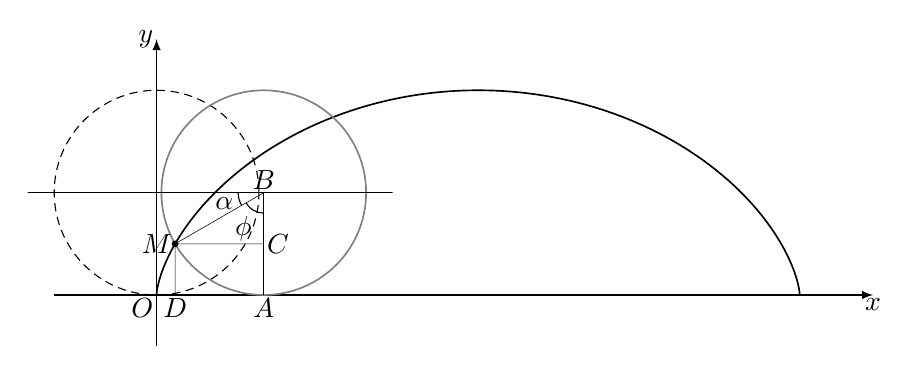
\begin{tikzpicture}[>=latex,scale=1.3,inner sep=1pt]
  \tkzDefPoints{0/0/O,0/1/O'}
  \tkzDefPoint({pi/3},0){A}
  \tkzDefPoint({pi/3},1){B}
  \tkzDefShiftPoint[B](-150:1){M}
  \tkzDefPointsBy[projection=onto O--A](M){D}
  \tkzDefPointsBy[projection=onto B--A](M){C}
  \draw[thin,->](-1,0)--(7,0)node[below]{$x$};
  \draw[thin,->](0,-0.5)--(0,2.5)node[left]{$y$};
  \draw[densely dashed](0,1)circle(1);
  \draw[semithick,domain=0:360,samples=200] plot ({\x/180*pi-sin(\x)},{1-cos(\x)});
  \tkzDrawCircle[semithick](B,M)
  \tkzDrawSegments(A,B B,M M,C M,D)
  \tkzDrawLine[add = 1.2 and 1.2](B,O')
  \tkzMarkAngle[size=0.2](M,B,C)
  \tkzLabelAngle[pos=0.4](M,B,C){$\phi$}
  \tkzMarkAngle[size=0.25](O',B,M)
  \tkzLabelAngle[pos=0.4](O',B,M){$\alpha$}
  \tkzDrawPoints[fill=black](M)
  \tkzLabelPoints[below left](O)
  \tkzLabelPoints[above](B)
  \tkzLabelPoints[below](A,D)
  \tkzLabelPoints[left](M)
  \tkzLabelPoints[right](C)
\end{tikzpicture}
\end{document}